\chapter{Évaluation Expérimentale}
\label{cp:evaluation}

Afin de valider les performances de notre stratégie, nous avons utilisé un script \texttt{sh}, qui permet de lancer plusieurs parties et de récupérer les résultats.
Ce script nous renvoie, pour un niveau donné et un nombre de parties donné, le pourcentage de victoires, le nombre moyen de déplacements effectués par le runner et le nombre moyen de bombes utilisées.

\section{Niveau 0}

\subsection{Résultats}

\begin{table}[!htpb]
    \begin{tabularx}{\textwidth}{lXXX}
        \toprule
        Pourcentage de victoires & Moyenne de déplacements & Moyenne de bombes \\
        \midrule
        100\% & 87.0 & 0.0 \\
        \bottomrule
    \end{tabularx}
    \caption{Résultats pour le niveau 0 sur 1000 parties}
    \label{tab:res-niveau-0}
\end{table}

\subsection{Analyse des défaites}

Il n'y a pas de défaites pour le niveau 0 et le nombre moyen de déplacements est entier, car n'y a pas d'ennemi, le runner prend toujours le même chemin.

\newpage

\section{Niveau 1}

\subsection{Résultats}

\begin{table}[!htpb]
    \begin{tabularx}{\textwidth}{lXXX}
        \toprule
        Pourcentage de victoires & Moyenne de déplacements & Moyenne de bombes \\
        \midrule
        100\% & 125.0 & 0.0 \\
        \bottomrule
    \end{tabularx}
    \caption{Résultats pour le niveau 1 sur 1000 parties}
    \label{tab:res-niveau-1}
\end{table}

\subsection{Analyse des défaites}

Il n'y a pas de défaites pour le niveau 1 et le nombre moyen de déplacements est entier.
Pourtant il y a un ennemi, mais le runner le contourne, et prend toujours le même chemin.
\newline
On remarque que la seule mécanique qui rend le jeu non déterministe est la position des ennemis lorsqu'ils réapparaissent.
Or, la solution que trouve notre stratégie est de contourner les ennemis, donc si elle réussi le niveau une fois, elle le réussira toujours.

\section{Niveau 2}

\subsection{Résultats}

\begin{table}[!htpb]
    \begin{tabularx}{\textwidth}{lXXX}
        \toprule
        Pourcentage de victoires & Moyenne de déplacements & Moyenne de bombes \\
        \midrule
        100\% & 174.0 & 0.0 \\
        \bottomrule
    \end{tabularx}
    \caption{Résultats pour le niveau 2 sur 1000 parties}
    \label{tab:res-niveau-2}
\end{table}

\subsection{Analyse des défaites}

Il n'y a pas de défaites pour le niveau 2, pour les mêmes raisons que pour le niveau 1.

\newpage

\section{Niveau 3}

\subsection{Résultats}

\begin{table}[!htpb]
    \begin{tabularx}{\textwidth}{lXXX}
        \toprule
        Pourcentage de victoires & Moyenne de déplacements & Moyenne de bombes \\
        \midrule
        98.2\% & 161.7 & 2.7 \\
        \bottomrule
    \end{tabularx}
    \caption{Résultats pour le niveau 3 sur 10000 parties}
    \label{tab:res-niveau-3}
\end{table}

\subsection{Analyse des défaites}

Malgré un pourcentage de victoires élevé, il y a des défaites pour le niveau 3.	Analysons une de ces défaites.

\begin{figure}[!htpb]
    \centering
    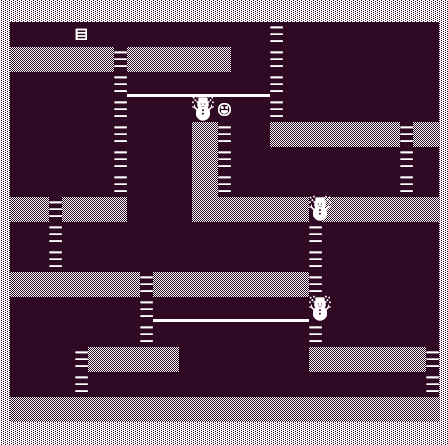
\includegraphics[width=0.5\textwidth]{Figures/level3-over.png}
    \caption{Défaite pour le niveau 3.}
    \label{fig:defaite-niveau-3}
\end{figure}

À cette position, le runner joue \texttt{DOWN}, ce qui le coince entre deux ennemis, l'empêchant d'avoir le temps ou l'espace nécessaire pour utiliser ses bombes. En mode debug, on constate que c'est le mode de rapprochement qui était activé.
\newline
À ce moment, il ne reste qu'un seul bonus, mais il est inatteignable car les ennemis bloquent tous les chemins. Dans ce cas, il est normal que le mode de mouvement spécial soit utilisé. Cependant, le runner aurait dû se diriger vers la droite.
\newline
Cette situation résulte d'une erreur : le mode de combat aurait dû être activé.

\newpage

\section{Niveau 4}

\subsection{Résultats}

\begin{table}[!htpb]
    \begin{tabularx}{\textwidth}{lXXX}
        \toprule
        Pourcentage de victoires & Moyenne de déplacements & Moyenne de bombes \\
        \midrule
        96.9\% & 189.4 & 1.5 \\
        \bottomrule
    \end{tabularx}
    \caption{Résultats pour le niveau 4 sur 10000 parties}
    \label{tab:res-niveau-4}
\end{table}

\subsection{Analyse des défaites}

Une des défaites les plus courantes pour le niveau 4 est la suivante :

\begin{figure}[!htpb]
    \centering
    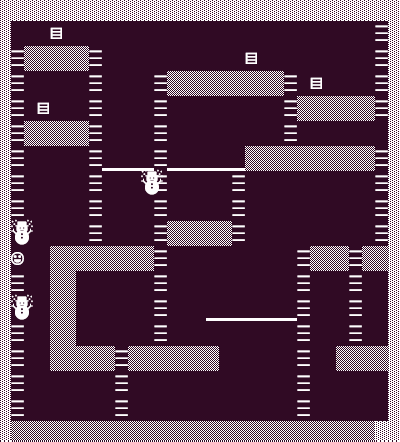
\includegraphics[width=0.4\textwidth]{Figures/level4-over.png}
    \caption{Défaite pour le niveau 4.}
    \label{fig:defaite-niveau-4}
\end{figure}

À cette position, le runner reste immobile, car il est bloqué entre deux ennemis.
Pourtant, il aurait pu jouer \texttt{RIGHT} pour se dégager.
\newline
Cette erreur provient du mode de mouvement en combat : lorsqu'un combat se déroule sur une échelle, le runner se limite à essayer de monter ou descendre.
Il aurait dû également envisager de se déplacer vers la gauche ou la droite pour se libérer.

\newpage

\section{Niveau supplémentaire}

Afin de tester notre stratégie sur un niveau plus difficile, nous avons créé un niveau supplémentaire.
Il reprend les mêmes plateformes que le niveau 3, mais avec des ennemis en plus.

\begin{figure}[!htpb]
    \centering
    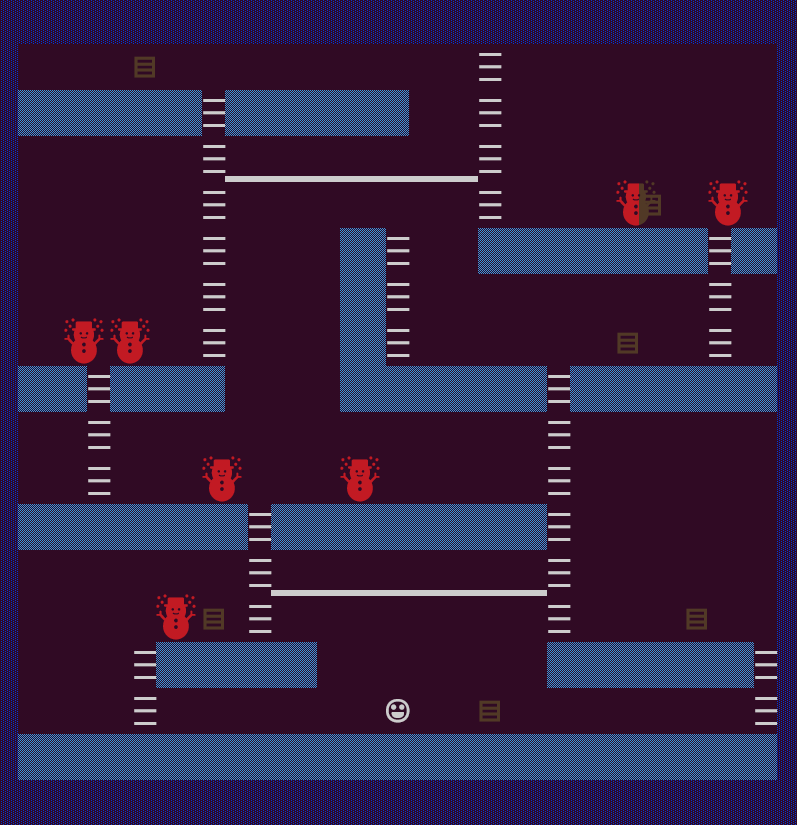
\includegraphics[width=0.4\textwidth]{Figures/level4.png}
    \caption{Niveau supplémentaire}
    \label{fig:niveau-supplementaire}
\end{figure}

\subsection{Résultats}

\begin{table}[!htpb]
    \begin{tabularx}{\textwidth}{lXXX}
        \toprule
        Pourcentage de victoires & Moyenne de déplacements & Moyenne de bombes \\
        \midrule
        50.9\% & 209.2 & 13.9 \\
        \bottomrule
    \end{tabularx}
    \caption{Résultats pour le niveau supplémentaire sur 1000 parties}
    \label{tab:res-niveau-supplementaire}
\end{table}

\subsection{Analyse des défaites}

Sur ce dernier niveau, il y a beaucoup de défaites, car il y a beaucoup d'ennemis.

\begin{figure}[!htpb]
    \centering
    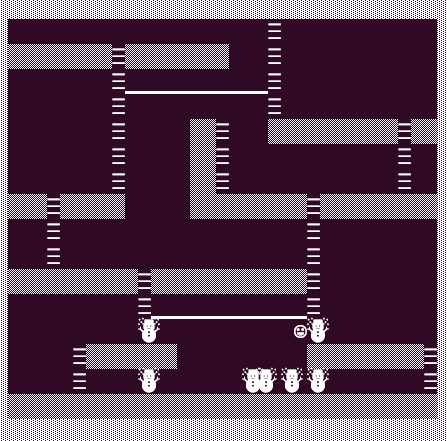
\includegraphics[width=0.4\textwidth]{Figures/level5-over.png}
    \caption{Défaite pour le niveau supplémentaire.}
    \label{fig:defaite-niveau-supplementaire}
\end{figure}

À cette position, le runner joue \texttt{DOWN}.
C'est un mouvement de combat qui vise, initialement, à ne pas combattre sur les cables, car on ne peut pas y poser de bombes.
De plus, il n'y a pas d'ennemi pile en dessous du runner, il joue donc \texttt{DOWN}.
\newline
C'est une erreur du mode de mouvement en combat, car le runner aurait dû se déplacer vers la gauche pour éviter les ennemis.

\section{Conclusion et persecpectives d'amélioration}

Notre stratégie a montré de bons résultats sur les premiers niveaux, mais elle a montré ses limites sur les niveaux plus difficiles.
\newline
Les erreurs proviennent principalement des modes de mouvement en combat, qui ne prennent pas en compte toutes les possibilités de déplacement.
\newline
C'est la limite de notre stratégie : elle ne peut pas prendre en compte toutes les situations possibles.
Il faudrait trouver un stratégie plus générale, qui ne prennent pas en compte des cas particuliers, mais qui soit capable de s'adapter à toutes les situations.
\newline
Je pense qu'estimer la position future des ennemis et l'utiliser dans A* pourrait être une piste d'amélioration.